\section{希格斯物理}
标准模型引入了一个具有非零真空期望值的复标量Higgs场,$\varphi$,其场势能项为:
\begin{equation}
 V(\varphi)=-v^2\lambda\varphi^{\dagger}\varphi+\lambda(\varphi^{\dagger}\varphi)^2
\end{equation}
其中,$v=(\sqrt{2}G_{F})^{-1/2}\approx246~$GeV为Higgs场真空期望值,$\lambda$是Higgs自耦合参数。通过自发对称性破缺,$W^{\pm}$和$Z$玻色子得到质量,
而且预言了一个额外的标量粒子,即Higgs玻色子。在标准模型中包含Higgs耦合项的拉氏量密度如公式\ref{eq:Higgs_Lagrangian}所示:
\begin{equation}
\label{eq:Higgs_Lagrangian}
\mathcal{L}=-\lambda\bar{f}fh+\delta_{V}V_{\mu}V^{\mu}(\lambda_{hVV}h+\lambda_{hhVV}h^2)+\lambda_{hh}h^2+\lambda_{hhh}h^3+\lambda_{hhhh}h^4
\end{equation}
其中,$f$代表费米子,$V$为$W^{\pm}$($\delta_{W}$=1)和$Z$($\delta_{Z}$=1/2)玻色子,并且方程中的耦合参数可以表达为:
\begin{equation}
 \begin{aligned}
 \lambda_{h\bar{f}f}=\frac{m_{f}}{v},~\lambda_{hVV}=\frac{2m_{V}^{2}}{v},~\lambda_{hhVV}=\frac{m_{V}^2}{v^2} \\
 \lambda_{hh}=\frac{m_{h}^2}{2},~\lambda_{hhh}=\frac{m_{h}^2}{2v}=\lambda v,~\lambda_{hhhh}=\frac{m_{h}^2}{8v^2}
 \end{aligned}
\end{equation}
Higgs质量模型并未预言,需要实验确定,当Higgs粒子质量确定之后,Higgs自耦合参数$\lambda_{hhh}$也随之确定,$\lambda_{hhh}$的测量是$hh$搜寻的首要目标。
还可以发现,Higgs与其他粒子的耦合强度依赖于粒子质量。

\subsection{单希格斯粒子产生模式}
在LHC单希格斯粒子可以有以下产生模式:
\begin{itemize}
 \item 胶子融合(ggF)$gg\rightarrow h$;
 \item 矢量玻色子融合(VBF)$q\prime{q}\rightarrow q\prime{q}h$;
 \item $W$或$Z$玻色子关联产生(Vh)$q\bar{q}\rightarrow Vh$,其中还包括部分($\sim$8\%)$gg\rightarrow Zh$(ggZh);
 \item 底夸克对关联产生($b\bar{b}h$)$q\bar{q}/gg\rightarrow b\bar{b}h$,和顶夸克对关联产生($t\bar{t}h$)$q\bar{q}/gg\rightarrow t\bar{t}h$;
 \item $t$过程单顶夸克关联产生($thqb$)$qg\rightarrow th\prime{q}b$(四味方案),和关联$W$玻色子产生($thW$)$gb\rightarrow thW$(五味方案);$s$过程可以忽略。
\end{itemize}
图\ref{fig:LHCHIGGSWG}分别总结了上述几种产生模式在$\sqrt{s}=13~$TeV时产生截面随$m_h$变化情况,和在$m_h$=125 GeV时随$\sqrt{s}$变化情况。
\begin{figure}[h]
\centering
 \begin{subfigure}[b]{0.45\textwidth}
  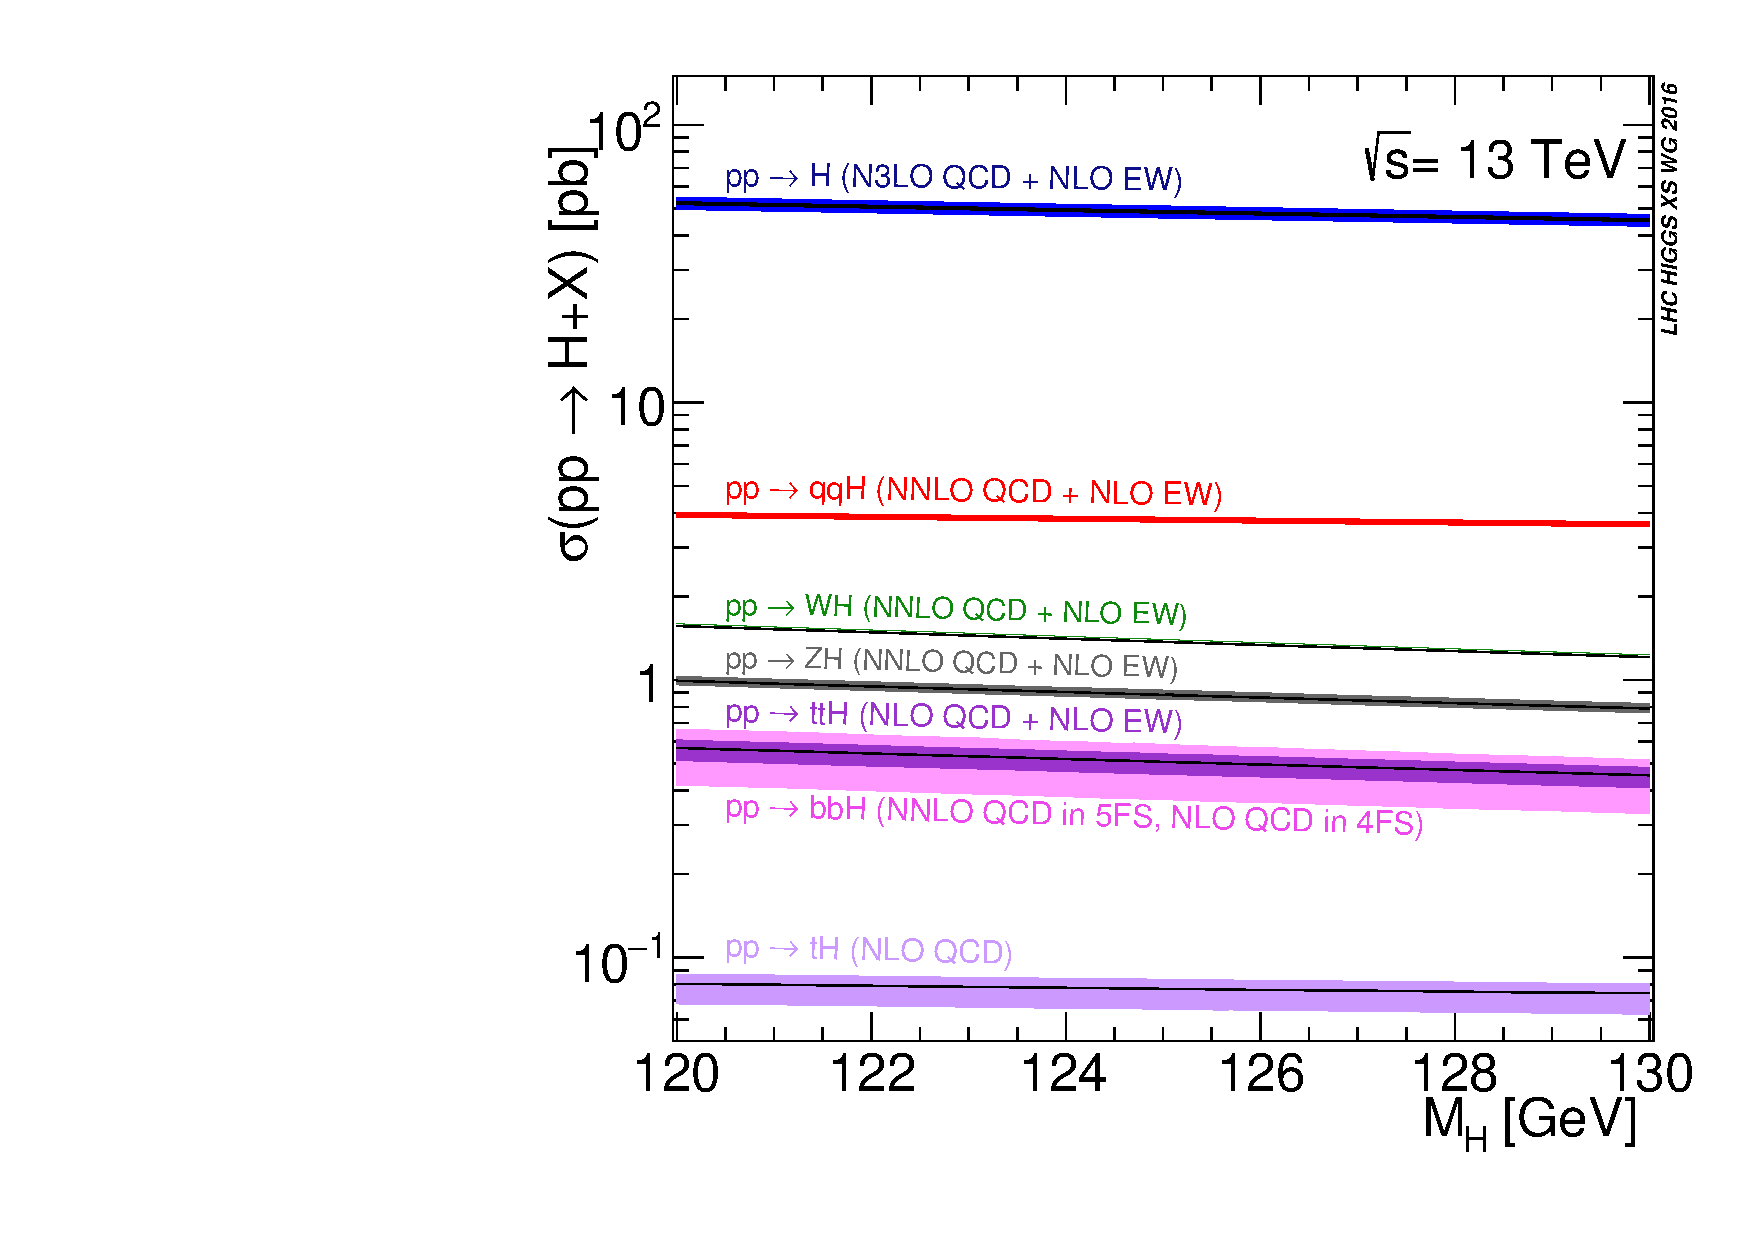
\includegraphics[width=0.75\textwidth,angle=-90]{fig/plot_13tev_H_sqrt.pdf}
  \caption{}
 \end{subfigure}
 \begin{subfigure}[b]{0.45\textwidth}
  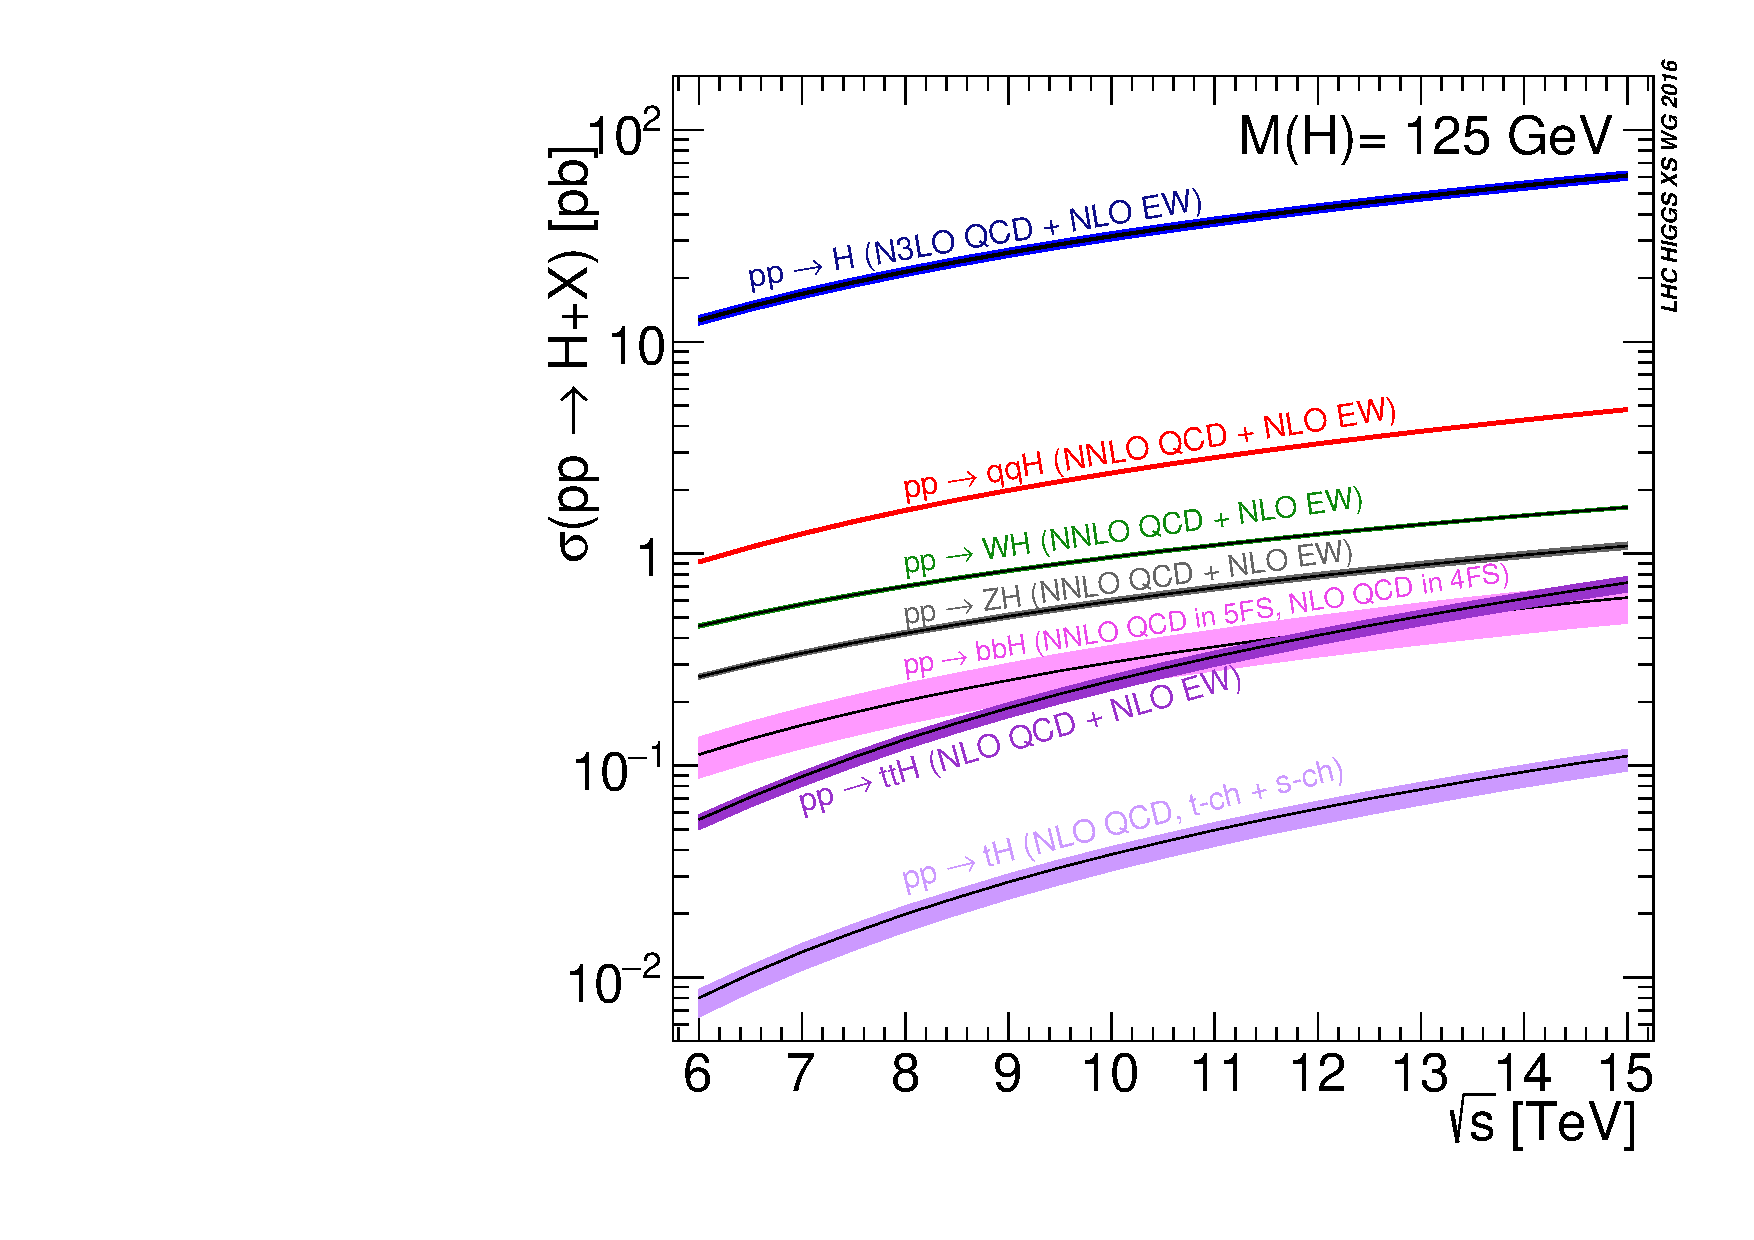
\includegraphics[width=0.75\textwidth,angle=-90]{fig/Plot_Escan_H125_new_sqrt.pdf}
  \caption{}
 \end{subfigure}
\caption{(a)标准模型希格斯粒子各产生模式截面随$m_h$变化($\sqrt{s}=13~$TeV),(b)标准模型希格斯粒子各产生模式截面随$\sqrt{s}$变化($m_h=125~$GeV)。}
\label{fig:LHCHIGGSWG}
\end{figure}
$ggF$是LHC上Higgs产生的主要过程,大约占比90\%($m_h$=125 GeV),是Higgs发现的首要贡献过程。在一般的超出标准模型设置中,$ggF$也假设为主要贡献过程,如本文将要
研究的$hh$产生。不过需要指出的是,$ggF$这过程有很高的QCD本底,不能很好地纯化。图\ref{fig:diagram_ggF}是$ggF$的领头阶(LO)的费曼图,因为胶子是无质量的,所以必须通过重味夸克传递。\\
$VBF$具有第二大的产生截面,其LO的费曼图如图\ref{fig:diagram_VBF}所示,除了产生Higgs外,还有两个较前向的喷注,这是它的显著信号特征,可以与$ggF$进行很好区分。
\begin{figure}[h]
\centering
 \begin{subfigure}[b]{0.45\textwidth}
  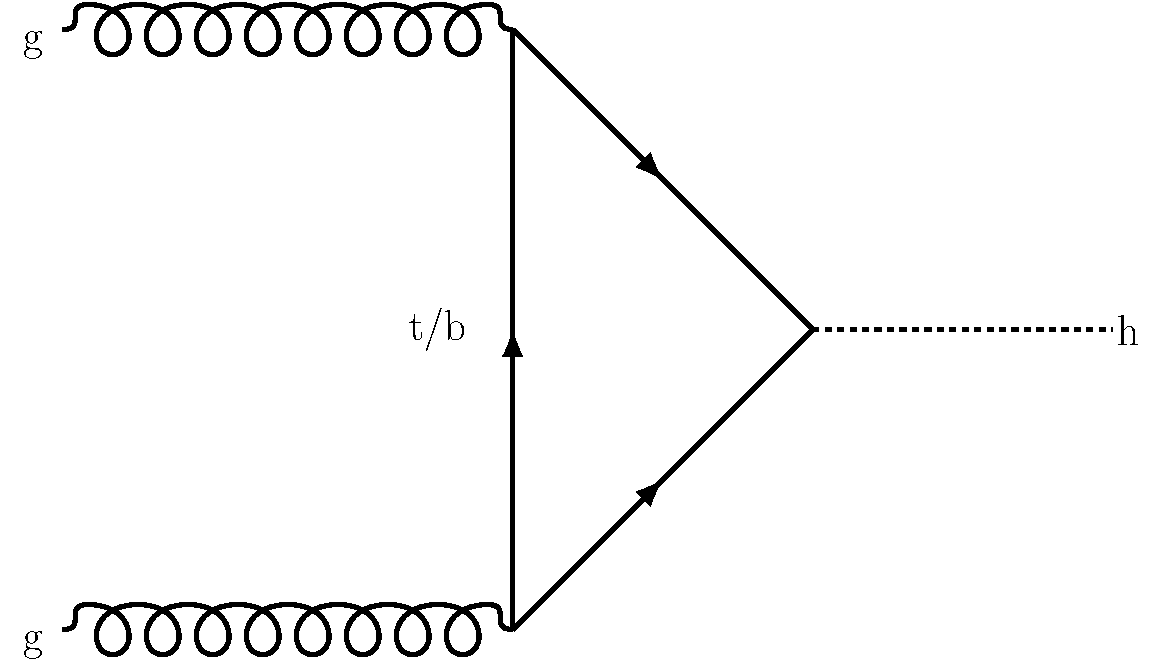
\includegraphics[width=0.75\textwidth]{fig/ggF.pdf}
  \caption{}
  \label{fig:diagram_ggF}
 \end{subfigure}
 \begin{subfigure}[b]{0.45\textwidth}
  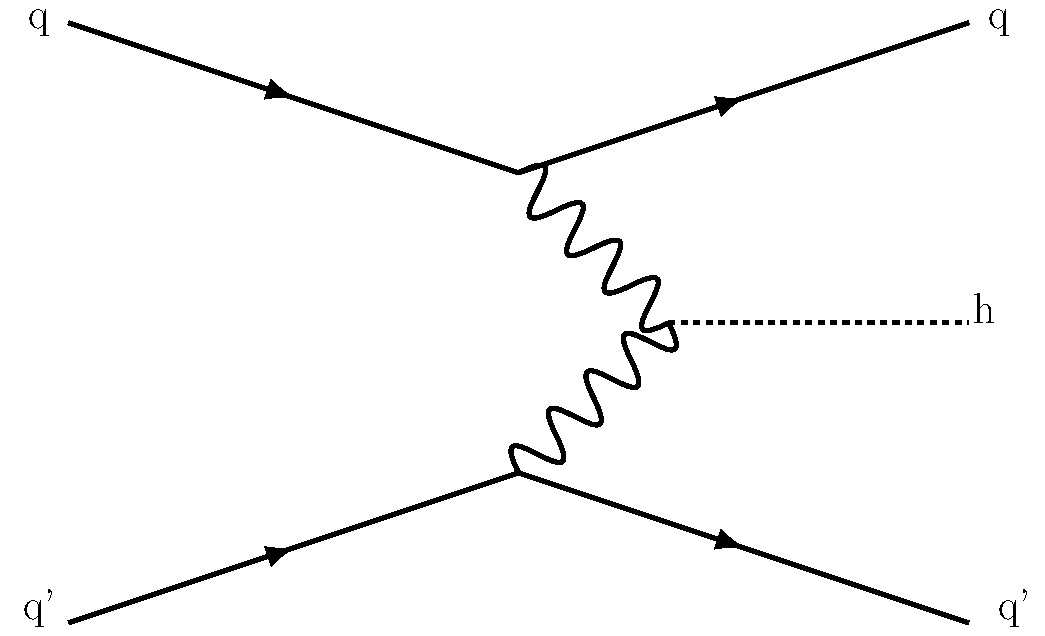
\includegraphics[width=0.75\textwidth]{fig/VBF.pdf}
  \caption{}
  \label{fig:diagram_VBF}
 \end{subfigure}
\caption{(a)典型LO阶$ggF$产生过程;(b)典型LO阶$VBF$产生过程。}
\label{fig:ggF_VBF}
\end{figure}
$Vh$过程的显著特征是末态中只有一个$W$或$Z$玻色子和Higgs,其LO阶费曼图如图\ref{fig:diagram_VH}所示。它可以通过玻色子的轻子化衰变产物去寻找,从而极大地压低QCD本底。
$Vh$是发现$h\rightarrow b\bar{b}$的黄金过程,并已于2018年正式发现\cite{Aaboud:2018zhk,Sirunyan:2018kst}。
通过$Vh$过程,我们还可以测量$\lambda_{hVV}$参数。另外,$ggZh$的产生截面很小,一般在的Higgs性质测量中,没有考虑。\\
\begin{figure}[h]
\centering
 \begin{subfigure}[b]{0.33\textwidth}
  
\includegraphics[width=0.85\textwidth]{fig/placeholder.pdf}
  \caption{}
  \label{fig:diagram_VH}
 \end{subfigure}
 \begin{subfigure}[b]{0.33\textwidth}
  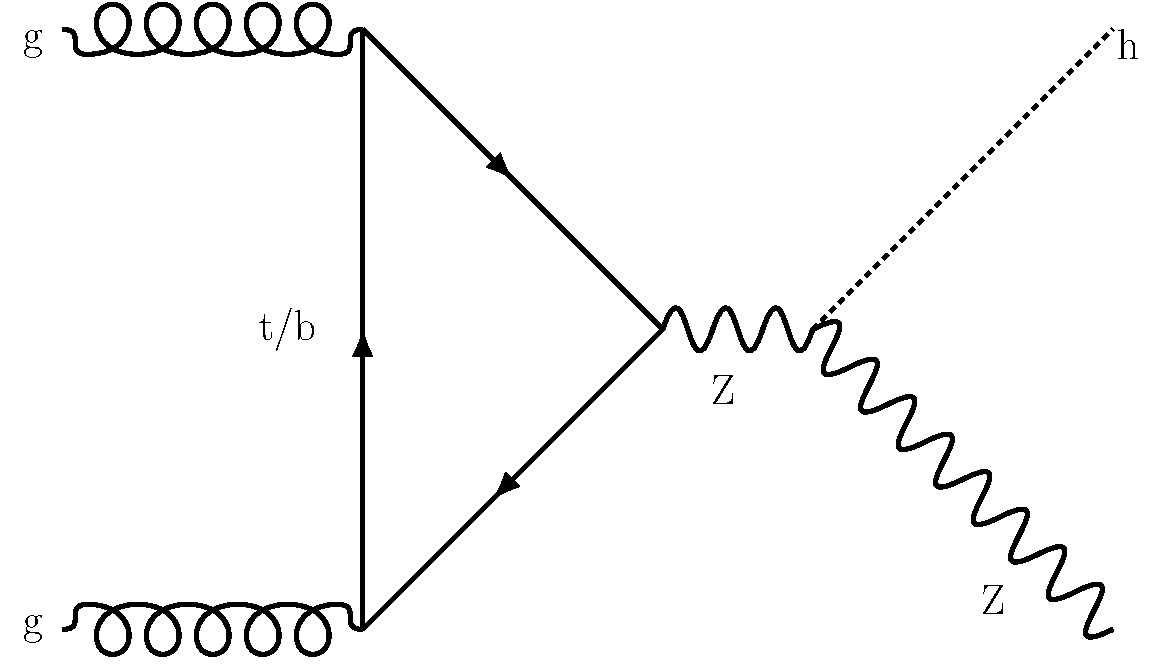
\includegraphics[width=0.85\textwidth]{fig/ggzh1_diagram.pdf}
  \caption{}
  \label{fig:diagram_ggzh1}
 \end{subfigure}
 \begin{subfigure}[b]{0.33\textwidth}
  
\includegraphics[width=0.85\textwidth]{fig/placeholder.pdf}
  \caption{}
  \label{fig:diagram_ggzh1}
 \end{subfigure}
\caption{(a)典型LO阶$Vh$产生过程;(b)(c)典型LO阶$ggZh$产生过程。}
\label{fig:Vh_ggZh}
\end{figure}

相比于$ggF$和$VBF$,$b\bar{b}h$和$t\bar{t}h$产生截面很小。对于$b\bar{b}h$,其挑战在于一般$b$夸克动量很低,不能有效地标记。而对于$t\bar{t}h$,得益于顶夸克的质量,
其衰变产物,如$b$喷注,具有较高的动量,可以有效标记,最终可以标记到此过程的相空间。通过$t\bar{t}h$的研究可以测量Higgs与最重粒子,$t$,的Yukawa耦合参数。
在ATLAS,$t\bar{t}h$是近几年的研究热点,已开展$t\bar{t}h(\rightarrow\gamma\gamma)$,$t\bar{t}h(\rightarrow b\bar{b})$以及$t\bar{t}h(\rightarrow \ell/\tau)$(一般称为tthML),
其中tthML研究将在本文讲述。$t\bar{t}h$的LO费曼图见图\ref{fig:diagram_tth}。\\
\begin{figure}[h]
\centering
 \begin{subfigure}[b]{0.33\textwidth}
  
\includegraphics[width=0.85\textwidth]{fig/placeholder.pdf}
  \caption{}
 \end{subfigure}
 \begin{subfigure}[b]{0.33\textwidth}
  
\includegraphics[width=0.85\textwidth]{fig/placeholder.pdf}
  \caption{}
 \end{subfigure}
 \begin{subfigure}[b]{0.33\textwidth}
  
\includegraphics[width=0.85\textwidth]{fig/placeholder.pdf}
  \caption{}
 \end{subfigure}
\caption{典型LO阶$t\bar{t}h$和$b\bar{b}h$费曼图。}
\label{fig:diagram_tth}
\end{figure}

$th$过程,具有最小的产生截面,其LO阶费曼图如图\ref{fig:diagram_th}所示。它的末态产物跟$t\bar{t}h$很相似,可以跟$t\bar{t}h$一起研究,联合测量Higgs与顶夸克的Yukawa耦合常数。\\
\begin{figure}[h]
\centering
 \begin{subfigure}[b]{0.33\textwidth}
  
\includegraphics[width=0.85\textwidth]{fig/placeholder.pdf}
  \caption{}
  \label{fig:diagram_VH}
 \end{subfigure}
 \begin{subfigure}[b]{0.33\textwidth}
  
\includegraphics[width=0.85\textwidth]{fig/placeholder.pdf}
  \caption{}
  \label{fig:diagram_ggzh1}
 \end{subfigure}
 \begin{subfigure}[b]{0.33\textwidth}
  
\includegraphics[width=0.85\textwidth]{fig/placeholder.pdf}
  \caption{}
  \label{fig:diagram_ggzh1}
 \end{subfigure}
 \begin{subfigure}[b]{0.33\textwidth}
  
\includegraphics[width=0.85\textwidth]{fig/placeholder.pdf}
  \caption{}
  \label{fig:diagram_ggzh1}
 \end{subfigure}
\caption{(a)(b)典型LO阶$thqb$过程;(c)(d)典型LO阶$thW$过程。}
\label{fig:diagram_th}
\end{figure}

表\ref{tab:xs_single_higgss_prod}总结这些产生过程在$\sqrt{s}=13~$TeV时的截面,其计算QCD阶数和QED阶数也列出。
\begin{table}[h]
\centering
\scalebox{0.75}{
\begin{tabular}{ccc}
\hline
\hline
Production porcess   &Cross section [pb]    &Order of calculation \\
\hline
$ggF$   &48.61+$(\text{theory})^{+4.27\%}_{-6.49\%}(\text{PDF})^{+1.85\%}_{-1.85\%}(\alpha_s)^{+2.59\%}_{-2.62\%}$   &N$^3$LO QCD + NLO EW  \cite{XSWG13TeV_2019,Cepeda:2019klc}\\
$VBF$   &3.766+$(\text{scale})^{+0.43\%}_{-0.33\%}(\text{PDF}+\alpha_s)^{+2.1\%}_{-2.1\%}$   &NNLO QCD +  NLO EW \cite{XSWG13TeV_2019,Cepeda:2019klc} \\
$Wh$   &1.358+$(\text{scale})^{+0.51\%}_{-0.51\%}(\text{PDF}+\alpha_s)^{+1.35\%}_{-1.35\%}$   &NNLO QCD + NLO EW \cite{XSWG13TeV_2019,Cepeda:2019klc}  \\
$Zh$   &0.880+$(\text{scale})^{+3.50\%}_{-2.68\%}(\text{PDF}+\alpha_s)^{+1.65\%}_{-1.65\%}$    &NNLO QCD + NLO EW \cite{XSWG13TeV_2019,Cepeda:2019klc} \\
%$ggZh $    &    &  \\
$t\bar{t}h$  &0.507+$(\text{scale})^{+5.8\%}_{-9.2\%}(\text{PDF}+\alpha_s)^{+3.6\%}_{-3.6\%}$    &NLO QCD + NLO EW \cite{XSWG13TeV} \\
%$th$  &    &NLO QCD  \\
$b\bar{b}h$  &0.486+$(\text{scale}+\text{PDF}+\alpha_s)^{+20.1\%}_{-23.9\%}$   &5FS NNLO + 4FS NLO \cite{XSWG13TeV} \\
%\hline
%Total    &    &  \\ 
\hline
\hline
\end{tabular}}
\caption{13 TeV质心系能量下标准模型希格斯玻色子(假设$m_h$= 125.09 GeV)产生截面理论预测值(pb),其中误差包括来自QCD scales, PDF以及$\alpha_s$的不确定度。}
\label{tab:xs_single_higgss_prod}
\end{table}

\subsection{标准模型希格斯对产生}
标注模型还预言了希格斯对产生,与单Higgs产生类似,其主要来源是胶子融合过程。在LHC LO阶的产生过程如图\ref{fig:diagram_SMhh_ggF}所示,分为箱图(\ref{fig:diagram_SMhh_box})和能够测量$\lambda_{hhh}$的三角图(\ref{fig:diagram_SMhh_triangle})。
在三角图中,中间态的Higgs作为一个传播子,质量不在壳,而末态的双Higgs均在壳;而中间态Higgs在壳,末态Higgs不在壳的情况被极大地压低\cite{Patrignani:2016xqp}\textbf{引用存疑}。
而且需要指出的是,箱图和三角图过程具有抵消干涉项,导致标准模型希格斯对总产生截面很小。
\begin{figure}[h]
\centering
 \begin{subfigure}[b]{0.45\textwidth}
  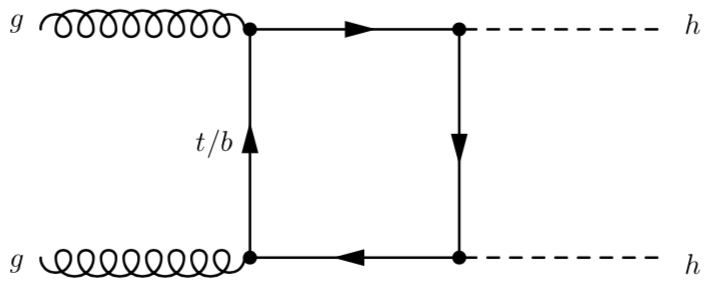
\includegraphics[width=0.85\textwidth]{fig/SMhh_box.png}
  \caption{}
  \label{fig:diagram_SMhh_box}
 \end{subfigure}
 \begin{subfigure}[b]{0.45\textwidth}
  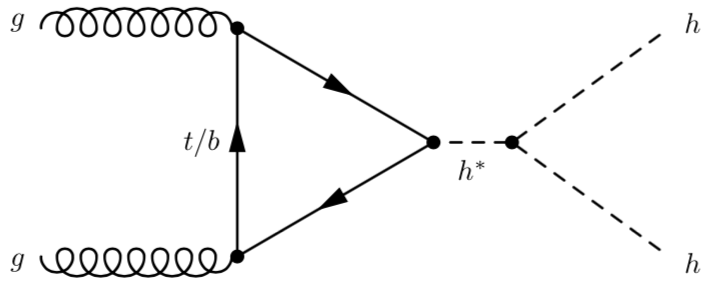
\includegraphics[width=0.85\textwidth]{fig/SMhh_triangle.png}
  \caption{}
  \label{fig:diagram_SMhh_triangle}
 \end{subfigure}
\caption{领头阶标准模型$hh$胶子融合产生过程。}
\label{fig:diagram_SMhh_ggF}
\end{figure}

另外,除了胶子融合过程,还有其他Higgs对产生模式,比如矢量玻色子融合,其领头阶费曼图如图\ref{fig:diagram_SMhh_VBF}所示。
需要指出的是,在ATLAS利用2015年和2016年进行的分析中,仅考虑了胶子融合过程,这也是本文$hh$研究的考虑范围,
但是在新一轮的研究中,一些分析道开始考虑矢量玻色子融合过程。
\begin{figure}[h]
\centering
  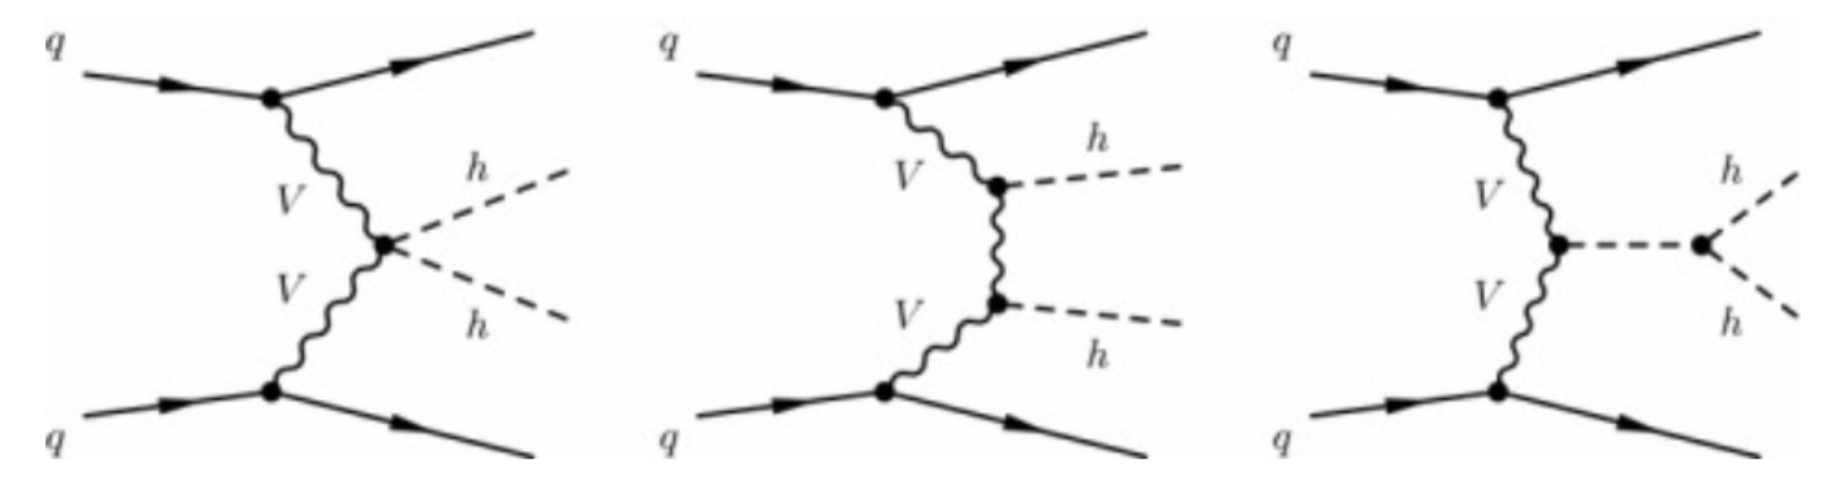
\includegraphics[width=0.85\textwidth]{fig/SMhh_VBF.png}
\caption{领头阶标准模型$hh$矢量玻色子融合产生过程。}
\label{fig:diagram_SMhh_VBF}
\end{figure}

图\ref{fig:diagram_SMhh_VBF}总结了不同$hh$产生过程截面随$\sqrt{s}$的变化情况。
\begin{figure}[h]
\centering
 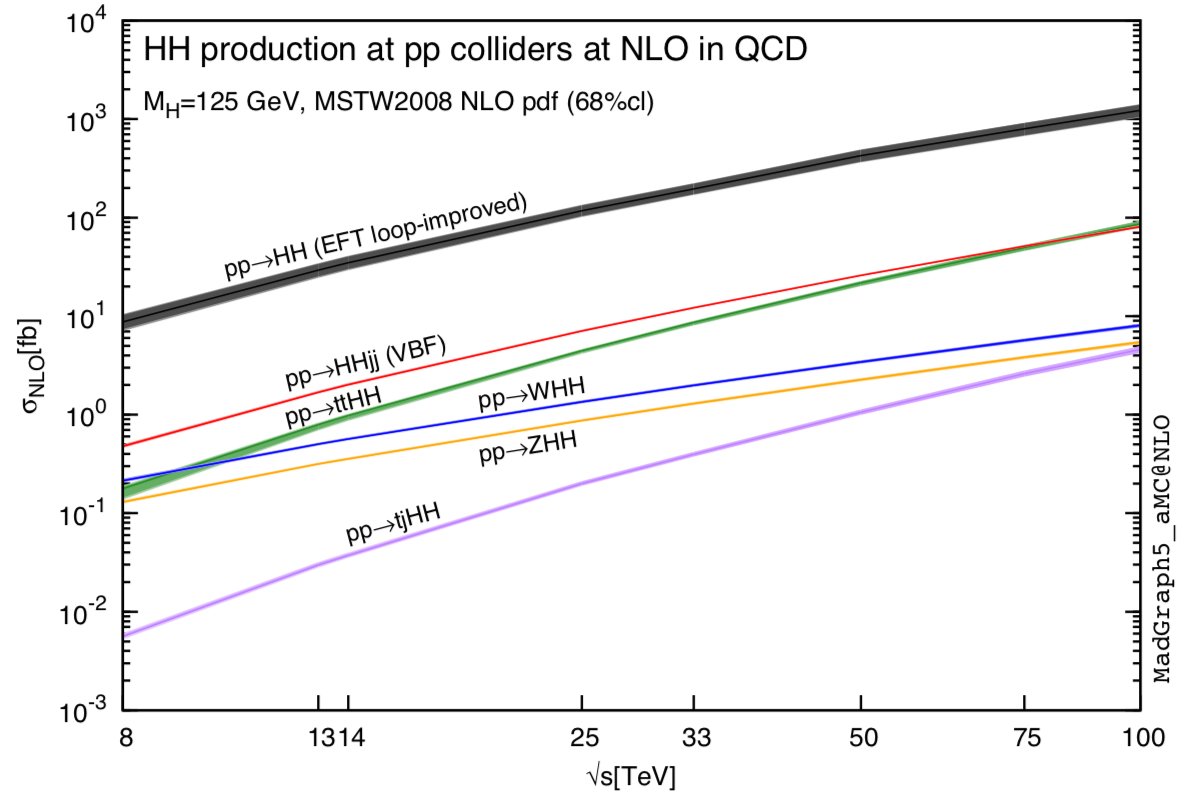
\includegraphics[width=0.85\textwidth]{fig/HH-xsec.png}
\caption{QCD次领头阶$hh$各产生模式的截面随$\sqrt{s}$变化情况\cite{Frederix:2014hta},包括胶子融合,矢量玻色子融合,顶夸克对,$W/Z$玻色子关联以及单顶夸克模式。
这里$H$指代标准模型Higgs,线宽代表不确定度,包括scale和PDF。}
\label{fig:diagram_SMhh_VBF}
\end{figure}
对于13 TeV质子质子对撞,考虑到QCD次次领头阶和次次领头阶对数求和,同时考虑到次领头阶有限顶夸克质量影响,几种$hh$产生过程的截面\cite{deFlorian:2016spz}总结如下\footnote{目前已有新的计算结果\cite{Grazzini:2018bsd,deFlorian:2013jea},但本文$hh$分析使用所列出的计算值。}:
%其中第一项误差是scale,第二项代表顶夸克质量影响,第三项是QCD耦合常数,第四项是PDF影响。
\begin{itemize}
 \item 胶子融合:$\sigma_{gg\rightarrow hh}=33.49^{4.3\%}_{-6.0\%}\pm5\%\pm2.3\%\pm2.1\%$;
 \item 矢量玻色子融合:$\sigma_{gg\rightarrow hh}=33.49^{4.3\%}_{-6.0\%}\pm5\%\pm2.3\%\pm2.1\%$;
 \item 胶子融合产生三Higgs:
\end{itemize}

\subsection{超出标准模型希格斯对产生}
虽然目前Higgs的测量结果越来越符合标准模型预期,但125 GeV的质量会有精细调节问题\cite{},如果有TeV量级的新粒子,不自然的问题就解决了。
在许多超出标准模型中,$hh$产生截面既可以通过非共振态也可以通过共振态模式增强。
对于非共振态模式中,可以通过修改$\lambda_{h\bar{t}t}$顶点\cite{Grober:2010yv,Contino:2012xk}或者一个新的带色荷标量粒子\cite{Kribs:2012kz};
还可以通过增强$\lambda_{hhh}$自耦合顶点,如图~\ref{fig:BSMhh_triangle}
中的绿圈所示。非共振态增强可以表述为超出标准模型产生截面与标准模型产生截面比值,对于希格斯自耦合顶点增强而言,等价于耦合常数增强,
即$\kappa_{\lambda}=\lambda/\lambda_{SM}$,从标准模型电弱测量得知,其被限制在$(-14, 17.4)$\cite{Kribs:2017znd}范围内。而且值得指出的是,
不同的$\kappa$对希格斯对产生有不同的影响\cite{Frederix:2014hta},图\ref{fig:HH_xs_kappa_14TeV}展示希格斯对产生截面随$\kappa$的变化情况。
在高$\lambda$区($|\kappa_{\lambda}|>10$),非共振态干涉贡献主要来自于自耦合顶点。
$\kappa$的确认可以通过测量希格斯对产生截面得到,这是$hh$研究的重要目标。
\begin{figure}[h]
\centering
 \begin{subfigure}[b]{0.33\textwidth}
  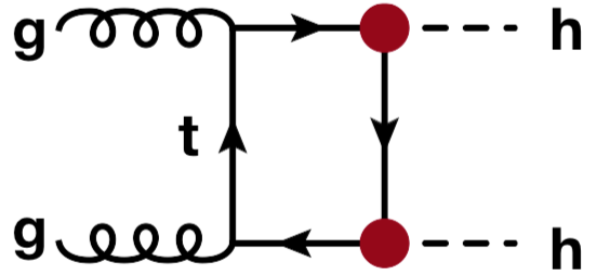
\includegraphics[width=0.85\textwidth]{fig/BSM_hh1.png}
  \caption{}
  \label{fig:BSMhh_box}
  \label{fig:diagram_BSMhh_box}
 \end{subfigure}
 \begin{subfigure}[b]{0.33\textwidth}
  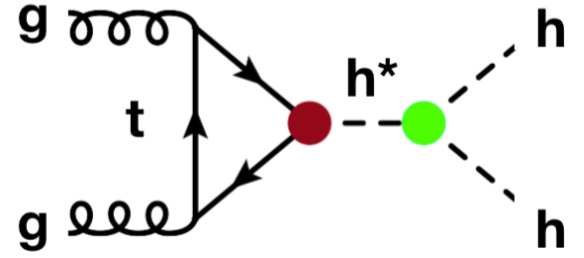
\includegraphics[width=0.85\textwidth]{fig/BSM_hh2.png}
  \caption{}
  \label{fig:BSMhh_triangle}
  \label{fig:diagram_BSMhh_triangle}
 \end{subfigure}
 \begin{subfigure}[b]{0.33\textwidth}
  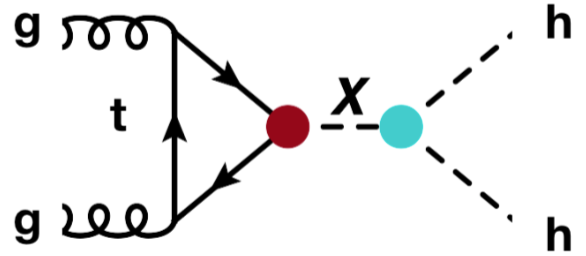
\includegraphics[width=0.85\textwidth]{fig/BSM_hh3.png}
  \caption{}
  \label{fig:BSMhh_resonance}
 \label{fig:diagram_resonant_hh}
 \end{subfigure}
\caption{超出标准模型希格斯粒子产生模式,其中\ref{fig:BSMhh_box}和\ref{fig:BSMhh_triangle}通过修改希格斯粒子耦合顶点常数实现,\ref{fig:BSMhh_resonance}则通过中间态高质量粒子,$X$,实现。}
\label{fig:diagram_BSM_hh}
\end{figure}

\begin{figure}[h]
\centering
 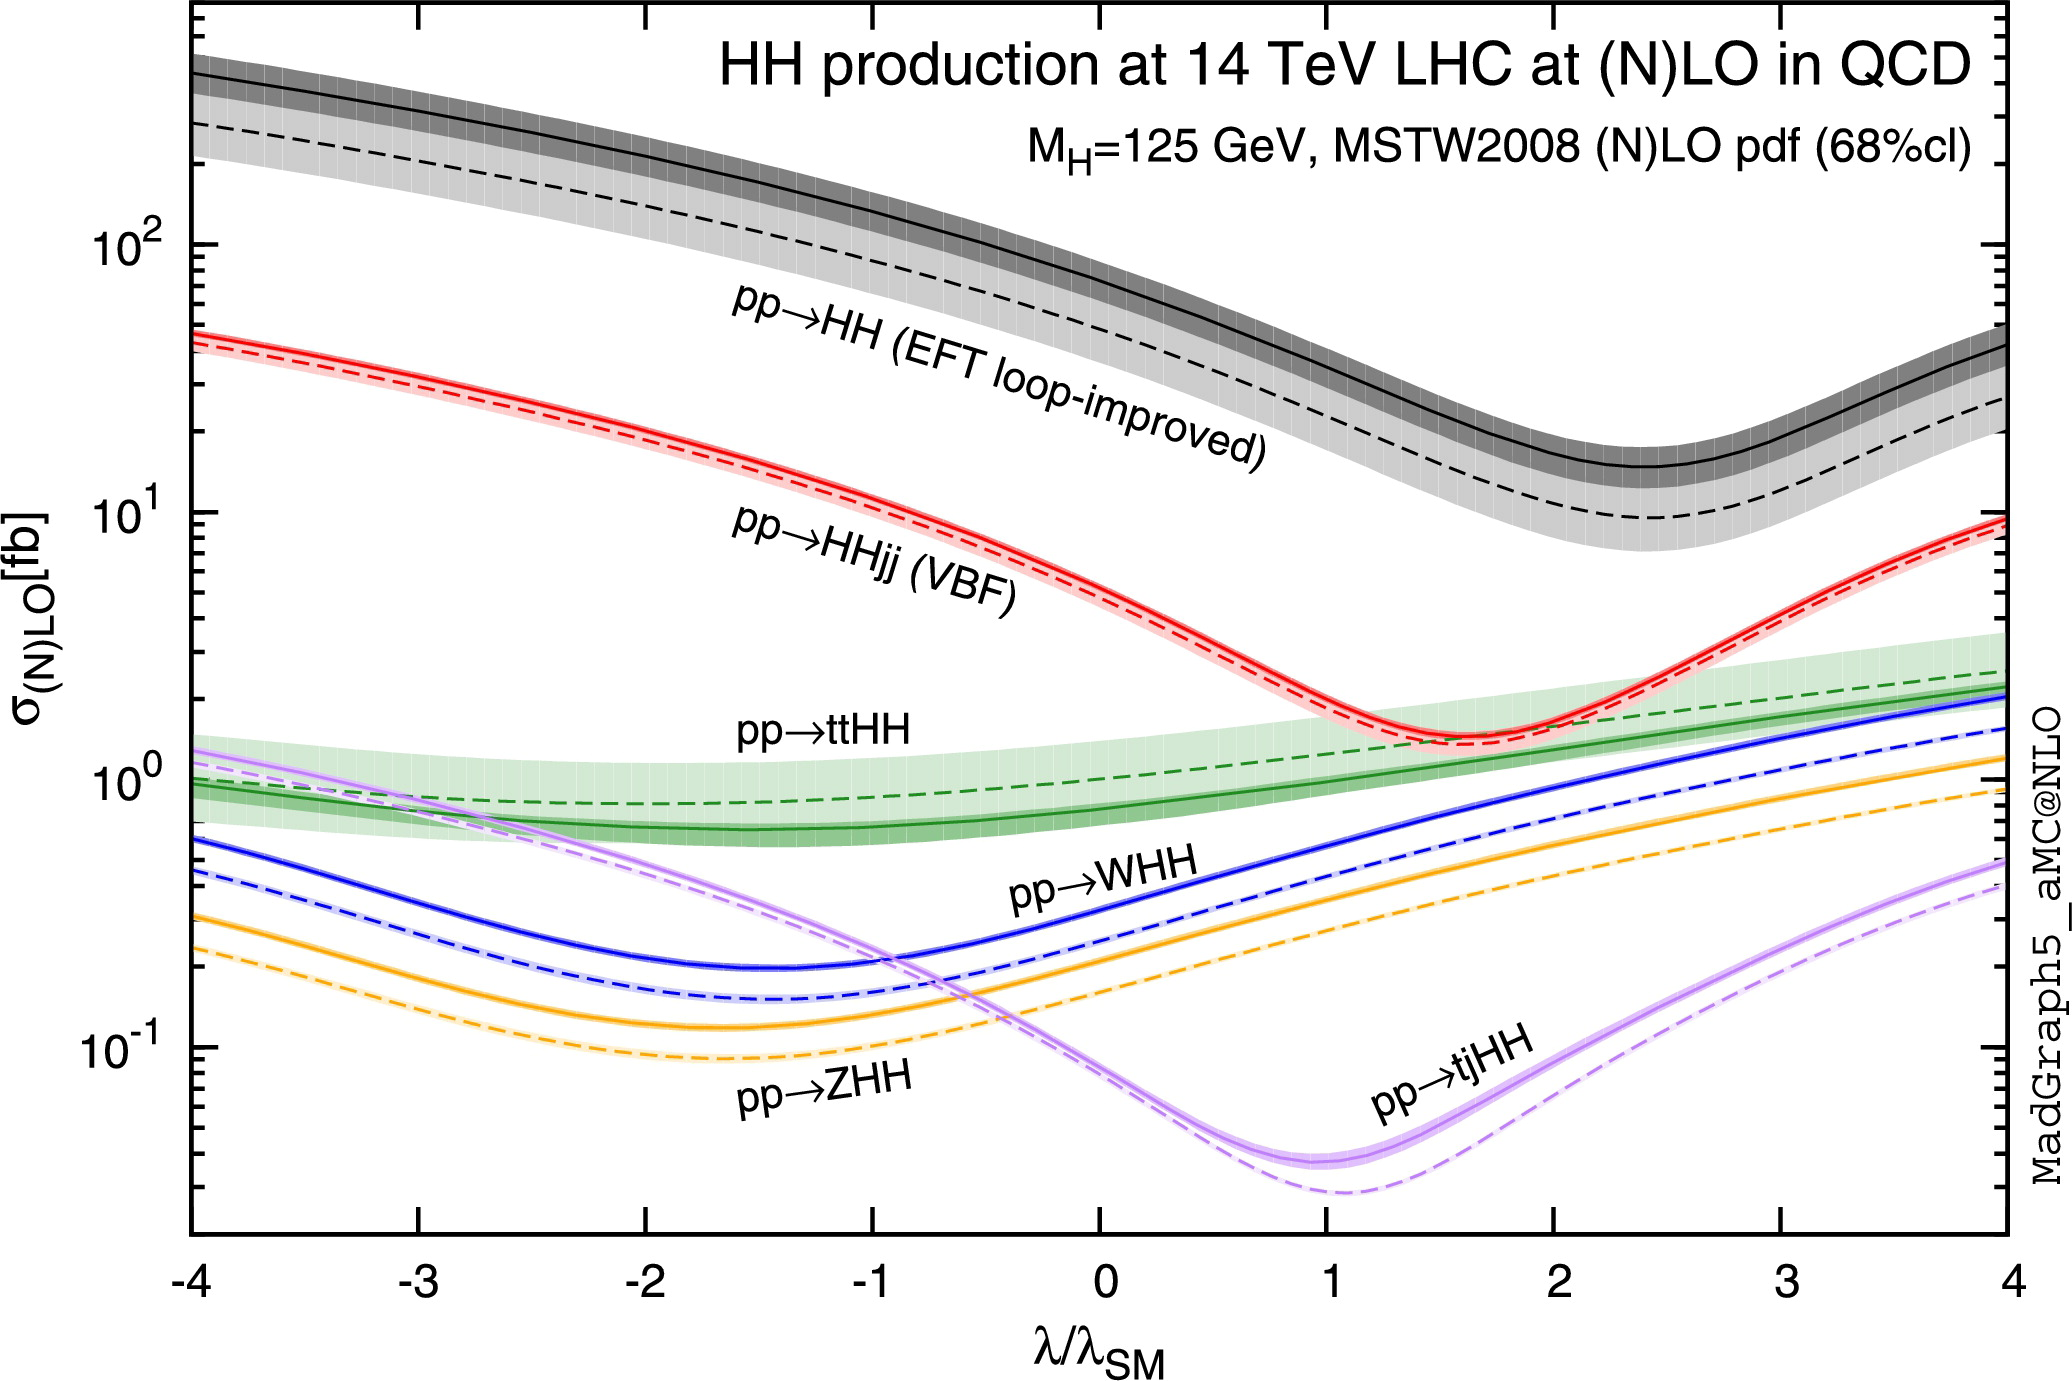
\includegraphics[width=0.85\textwidth]{fig/HH_xs_kappa_14TeV.jpg}
  \caption{14 TeV质心系能量下希格斯粒子对QCD(次)领头阶的产生截面随自耦合系数的变化情况,其中浅色虚线(深色实线)对应 领头阶 (次领头阶) 结果,其线宽代表来自scales和PDF的系统误差。 
  $kappa$=1表示标准模型希格斯对产生。}
  \label{fig:HH_xs_kappa_14TeV}
\end{figure}

理论上比较容易引入一个新的与希格斯粒子耦合的标量粒子,从而使得希格斯对产生截面增大。一个简单的扩展是2HDM~\cite{2HDMTheory},它有两个希格斯二重态,
从而有5个希格斯玻色子,分别是$h$(轻标量Higgs,一般看作发现的标准模型Higgs),$X$(重标量Higgs),$A$(重赝标量Higgs),$H^{\pm}$(两个带电Higgs)。
为了避免树图阶味道改变中性流,2HDM应用分立对称性使得带电费米子只与一个希格斯二重态耦合。

\subsection{希格斯对衰变}
希格斯粒子的寿命只有$1.56\times10^{-22}~$s,在对撞顶点即衰变,表\ref{fig:HH_br}总结了$hh$的主要衰变道的分支比。在\RunOne ,ATLAS研究过$b\bar{b}b\bar{b}$\cite{Aad:2015uka},
$b\bar{b}\gamma\gamma$~\cite{Aad:2014yja},$b\bar{b}\tau^{+}\tau^{-}$和$WW^{*}\gamma\gamma$,均没有观测到数据与预期的明显偏差。
对于非共振态模式,其截面上限为0.69 pb,对应$\kappa<$70。
共振态模式的联合拟合截面上限总结在图\ref{fig:HH_run1_combined}。
\begin{figure}[h]
\centering
 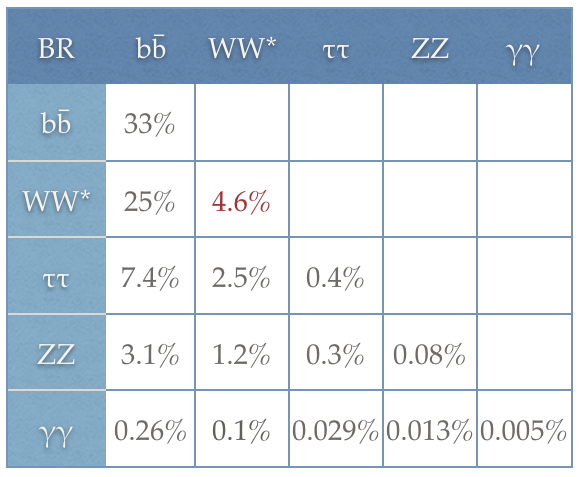
\includegraphics[width=0.75\textwidth]{fig/HH_br.png}
  \caption{$hh$主要衰变道分支比,计算时假设$m_h$=125 GeV。}
  \label{fig:HH_br}
\end{figure}

\begin{figure}[h]
\centering
 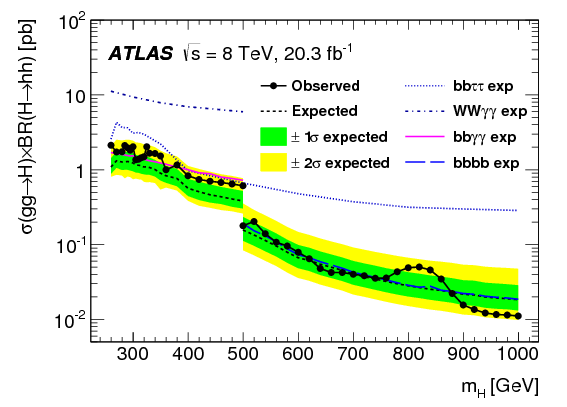
\includegraphics[width=0.85\textwidth]{fig/HH_run1_combined.png}
\caption{在8 TeV质心系能量时$\sigma(gg\rightarrow H)\times\text{BR}(H\rightarrow hh)$的95\%置信度下的观测上限值与期望上限值,结果联合拟合了$b\bar{b}\tau\tau$, $WW^*\gamma\gamma$, $b\bar{b}\gamma\gamma$以及$b\bar{b}b\bar{b}$分析道。绿色和黄色区分别表示期望上限值的$\pm 1\sigma$和$\pm 2\sigma$,500 GeV以上的提升得益于$b\bar{b}b\bar{b}$的加入。}
\label{fig:HH_run1_combined}
\end{figure}

现就一些衰变道作出简要概述:
\begin{itemize}
 \item $b\bar{b}b\bar{b}$:它具有最大的衰变分支比,是$hh$搜寻的主要分析道,能够重建Higgs以及$X$的质量,但是其分辨率受限于$b$喷注重建及鉴别。在低$m_X$区,
 因为$b$喷注触发效率太低,其显著性较低;但是在高$m_X$区,两个$b$喷注倾向合并,可以重建两个large-$R$~$b$喷注,而且得益于提高的$b$喷注触发效率,其显著性得到提高。
 \item $b\bar{b}W^{+}W^{-}$:具有第二大分支比,但是$t\bar{t}$本底限制了显著性,目前ATLAS正在积极研究优化策略。
 \item $b\bar{b}\gamma\gamma$:虽然截面不大,但是受益于较干净的双光子本底以及很好的光子分辨,在低$m_X$区有显著优势,
 但在高质量区,双光子的合并对光子鉴别造成影响,使得显著性下降。
 \item $b\bar{b}\tau^{+}\tau^{-}$:该道与前两个道具有相当的显著性,尤其是在低$m_X$区,其主要挑战是赝$\tau$的本底处理。
 \item $WW^{*}\gamma\gamma$:该道与上述衰变道相比具有较差的显著性,但是得益于双光子以及轻子化衰变的$W$玻色子,本底较少,是$hh$搜寻的重要补充。
 \item $WW^{*}WW^{*}$:该道是本文$hh$分析的研究题目,将在章节\ref{}详细讲述。
 \item $WW^{*}\tau\tau, \tau\tau\gamma\gamma, \tau\tau\tau\tau, b\bar{b}ZZ, WWZZ$:这些衰变道的分支比都很小,均不能或者部分重建Higgs,还未公开发表过结果。
 但是随着ATLAS累积更多的数据,使用单举策略\footnote{$WW^{*}\gamma\gamma$和$WW^{*}WW^{*}$也纳入其中},即以它们的衰变物进行分类,如轻子数,
 不明显关注$hh$衰变中间态,而后进行优化,最后联合拟合得出结果,也许可以为$hh$搜寻作出重要贡献。
\end{itemize}
